\usetikzlibrary{shapes}
\newcommand*\circled[1]{\tikz[baseline=(char.base)]{
            \node[shape=circle,draw,inner sep=2pt] (char) {#1};}}

\section{Visualization}
In this section, Ramu explains the parts of the project group he was responsible for, and how they affected the final version of the project. 

In this project group, my main task was to build a Graphical User Interface(GUI) enabling users to make transactions and visualize the Directed Acyclic Graph (DAG) - the core, using which the protocol of Asynchronous Blockchain without Consensus (ABC) works.  Table \ref{tab:ramu_resp_code} shows all parts of the project I was responsible for.


\begin{table}[htbp]
	\centering
	\begin{tabular}{ll}
		\hline
		\textbf{GitLab Repository} & \textbf{File Name} \bigstrut\\
		\hline
		abc\_protocol & zmq\_server.py \bigstrut[t]\\
		\hline
		gui-api & all \\
		\hline
        rotrans-web-gui & all \\
		\hline
	\end{tabular}%
	\caption{List of repositories or files created or maintained by Ramu}
	\label{tab:ramu_resp_code}%
\end{table}%

\subsection{Overview}
There are six major use cases and are illustrated in Figure \ref{fig:use_case}. Figure \ref{fig:ramu_highlevel_overview} illustrates a high-level abstraction of the working of the GUI and the Agent. There are three high-level components that are responsible for aggregating data from the Agent.

\begin{itemize}
	\item Web-GUI  
	\item API 
	\item Agent
\end{itemize}

\begin{figure}[htbp]
	\centering
	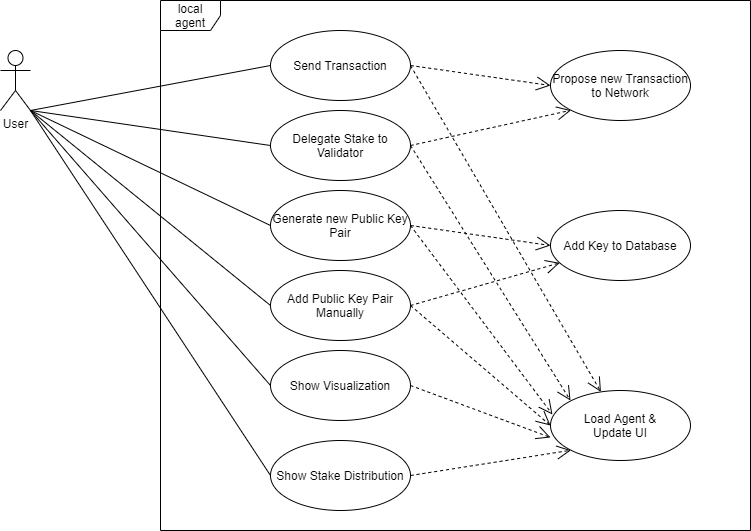
\includegraphics[width=0.8\textwidth, trim={0cm 0cm 0cm 0cm},clip]{figures/drawio/use_case.pdf}
	\caption{Use Case}
	\label{fig:use_case}
\end{figure}


\begin{figure}[htbp]
    \centering
    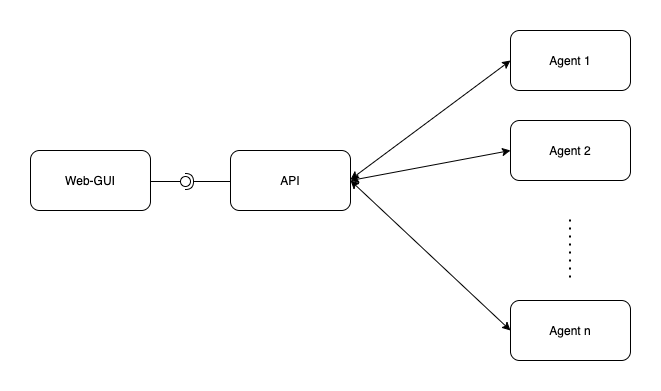
\includegraphics[width=0.8\linewidth]{figures/images/ramu/highlevel.png}
	\caption{High level workflow}
	\label{fig:ramu_highlevel_overview}
\end{figure}


\subsection{Web-GUI}
The GUI is developed using one of the most widely used JavaScript-based User Interface (UI) development frameworks, React. The actual code is written in Typescript (ES6 syntax) and is compiled into JavaScript (ES5 syntax) that can run on all the modern web browsers. Additionally, the Redux library is used for managing the state of the application. The application is build based on the Container-View pattern, one of the most widely used component-based UI development design patterns. Figure \ref{fig:ramu_gui_blocks} illustrates a complete breakdown of Web-GUI. A brief description of the low-level components is described below:

\begin{itemize}
	\item \textbf{Assets}: Comprises all the graphical assets used in the application inScalable Vector Graphics (SVG) format.
	\item \textbf{Components}: Bundles all the reusable components together. Components include balance indicator, button, menu bar, toolbar, dialog, error field, loading indicator, and text input. Each of the components has its own test file, component description file, and a Cascading Style Sheet (CSS).
	\item \textbf{Utils}: Comprises all the utility functions used throughout the application. Utility functions include validation for number inputs, validation for hexadecimal inputs, and conversion of the timestamp to a UTC time.
	\item \textbf{Core}: This module comprises the root reducer, root sagas, and root selectors.
	\item \textbf{Modules}: There are three modules: stake, transactions, and visualization. Each of the modules has its own set of actions, reducers, interfaces, sagas, and components. The components here are used only within the corresponding module and not with other modules.
\end{itemize}

\textbf{Application state management using Redux:} Redux is a store to manage the components and their associated states synchronously. Redux creates a set of procedures for the components to operate and interact with the store so that the components do not read or update the store in a random manner. The store can be accessed by all the components in a structured way through \textit{reducers} and \textit{actions}. A reducer function takes the previous state of the component and returns the next state for the same component. Every module under the \textbf{modules} directory of the \textit{rotrans-web-gui} repository has the following set of subdirectories: 
\begin{enumerate}
	\item actions
	\item components 
	\item interfaces
	\item reducers
	\item sagas
	\item selectors
\end{enumerate}
The \textit{index.tsx} file in the root of any directory is the starting point of the module/component. The \textit{components} directory contains the set of components that are used within a module. The \textit{actions} directory contains the redux actions that is been utilized by the components in the directory. The \textit{interfaces} directory holds all the Typescript interfaces that define the properties of the objects that are used by the component. The \textit{reducers} directory contains the module's reducer function that manipulates the state of the component. \textbf{Performing API calls using Redux Saga}: Redux works completely synchronous and performing side-effects (for example, making a call to the API to trigger key pair generation when the user clicks on \textit{Generate Keys} button) would actually block the UI making it unusable until a response is received from the API. In order to prevent this, the redux-saga library is used to execute the side-effects asynchronously. The files under the \textit{sagas} directory are actually defined to execute the side-effects. In order to perform the actual API calls, \textbf{fetch} API of JavaScript core is used. \textbf{Retrieving state using Selectors:} Selectors are functions that are defined to extract the state of the variables in the store and feed it to the components in the UI. The components that are used commonly by all the modules are placed under the \textit{src}$>$\textit{components} directory. Every component has its own \textit{index.tsx} file and an associated CSS style sheet \textit{styles.css}. All the components have a subdirectory named \textit{\_\_test\_\_} that contain unit test suites for the components.

\begin{figure}[htbp]
    \centering
    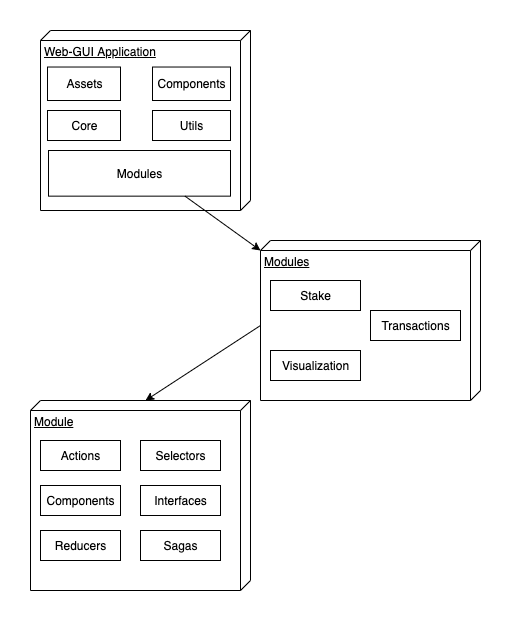
\includegraphics[width=0.5\linewidth]{figures/images/ramu/gui_block.png}
	\caption{Web-GUI Component Breakdown}
	\label{fig:ramu_gui_blocks}
\end{figure}

\subsection{The API}
The API is developed using Flask, a micro web framework for developing RESTful web services using Python. The API handles requests from the Web-GUI and chooses the right Agent to query for the data based on the provided port number. The port number is embedded in all of the requests from Web-GUI. Furthermore, the API is responsible for pre-processing the DAG to graphically visualize it in the UI. All the requests and responses with the Web-GUI and Agent are in JavaScript Object Notation (JSON) format. Figure \ref{fig:ramu_api_class} illustrates a class diagram representation of the API. The communication between the Web-GUI and the API happens through HyperText Transfer Protocol (HTTP) and the communication between the API and the Agent is established through ZeroMQ (ZMQ) sockets. The API acts as the ZMQ client (ZMQ Request socket) and every Agent is embedded with a ZMQ server (ZMQ Reply socket). According to the documentation of ZMQ, the request socket will block on send unless it has successfully received a reply from the reply socket.

\begin{figure}[htbp]
    \centering
    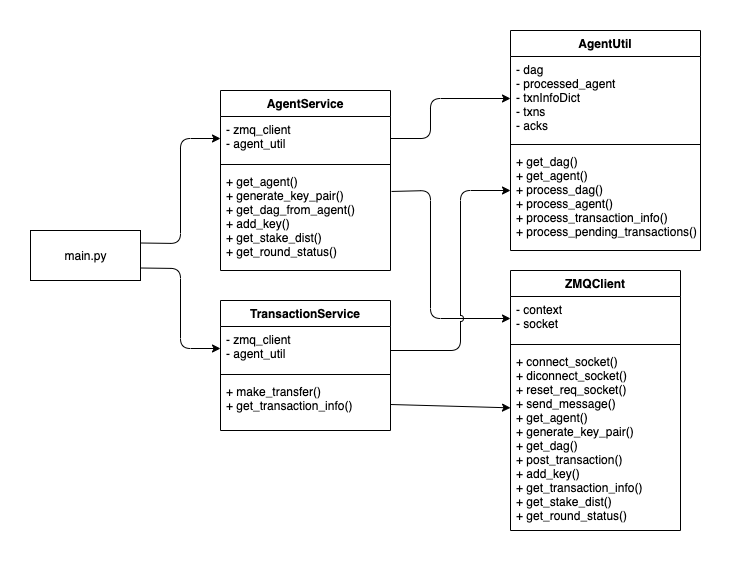
\includegraphics[width=0.9\linewidth]{figures/images/ramu/api_class.png}
	\caption{Class Diagram of API}
	\label{fig:ramu_api_class}
\end{figure}

The \textit{ZMQClient} class handles the requests that should be forwarded to the Agent. The \textit{send\_message()} function converts the request to a JSON format and transmits the request to the ZMQ reply socket (ZMQ.REP). The port of the reply socket is also specified as a parameter for the function to which the request socket connects to. The \textit{AgentUtil} class defines the functions for pre-processing the information before it is been transferred to the UI. The \textit{process\_agent()} function works on the agent object and generates a JSON for the transactions screen shown in Figure \ref{fig:ramu_ui_txn_screen}. The \textit{process\_dag()} function pre-process the DAG which is actually a list of dictionaries received from the \textit{LocalMessageHandler} class of the Agent. This function determines and differentiates the transactions, acks, and checkpoints and accordingly creates the nodes and edges as python dictionaries. These dictionaries are then converted to JSON and sent in the response body of the HTTP call to the UI. Unlike the ABC protocol, the prefix-tree in the agent does not contain unconfirmed transactions. These are maintained separately in \textit{pending\_transactions} in the \textit{Agent} class in abccore module. In order to visualize the unconfirmed transactions, the \textit{pending\_transactions} list is also fetched from the Agent, along with the DAG. The stake of an unconfirmed transaction is updated whenever this transactions receives acks from the validators. The \textit{process\_transaction\_info()} function aids in visualizing the most recent stake information of the unconfirmed transactions. 

\subsection{The Agent}
The Agent is embedded with a ZMQ server and this server responds to the requests from the API. This communication between the Agent and the API happens locally and not through the internet. The file \textbf{zmq\_server.py} in the Agent module defines the classes \textit{AgentUtil} and \textit{LocalMessageHandler}. A class diagram of the same is illustrated in Figure \ref{fig:ramu_agent_class}. The \textit{UIMessageHandler} initializes the ZMQ reply socket and starts listening for the requests from API. This is handled by the \textit{perform\_maintenance()} method overridden in the \textit{UIMessageHandler} class. According to the ZMQ documentation, the reply will block on receive unless it has received the request. Each request and reply is paired and has to be successful.

\begin{figure}[htbp]
    \centering
    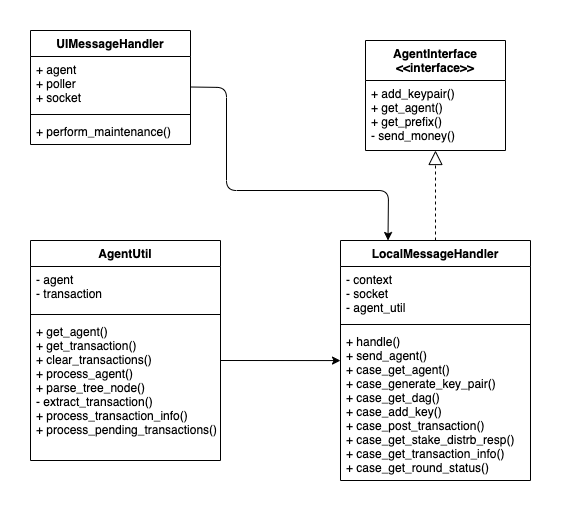
\includegraphics[width=0.9\linewidth]{figures/images/ramu/agent_class.png}
	\caption{Agent classes responsible for handling requests from API}
	\label{fig:ramu_agent_class}
\end{figure}

The \textit{LocalMessageHandler} class handles the requests from the API. Similar to the API, the requests and responses are in JSON format. The port of the server is configured in the \textit{self\_contact.json}. The \textit{AgentUtil} class defines functions for extracting information from the Agent. The notable function \textit{parse\_tree\_node()}, iterates over the prefix-tree and generates a list of dictionaries that contain transactions, acks, and checkpoints. A byte string cannot be transmitted as a JSON. Therefore, all the identifiers and keys are converted to respective hexadecimal strings. 

\subsection{User Interface (UI) Design}
The UI consists of three screens: visualization, transaction, and the stake distribution chart and are illustrated in Figure \ref{fig:ramu_ui_menu_bar}.

\begin{figure}[htbp]
    \centering
    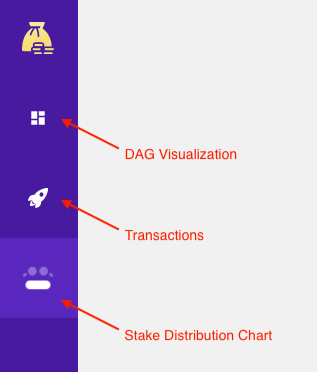
\includegraphics[width=0.3\linewidth]{figures/images/ramu/menubar.png}
	\caption{Menu Bar}
	\label{fig:ramu_ui_menu_bar}
\end{figure}

\subsubsection{Transactions}
A complete overview of transactions screen is shown in Figure ~\ref{fig:ramu_ui_txn_screen}. Typical use cases include: 
\begin{enumerate}
	\item Making a transfer to another agent (Figure \ref{fig:ramu_ui_transfer_mode} and \ref{fig:ramu_ui_delegate_mode}). The transaction value input field is validated for numbers with or without decimal digits, the public key field of the recipient, and the validator key is validated for a hexadecimal string.
	\begin{figure}[!htb]
		\minipage{0.45\textwidth}
		  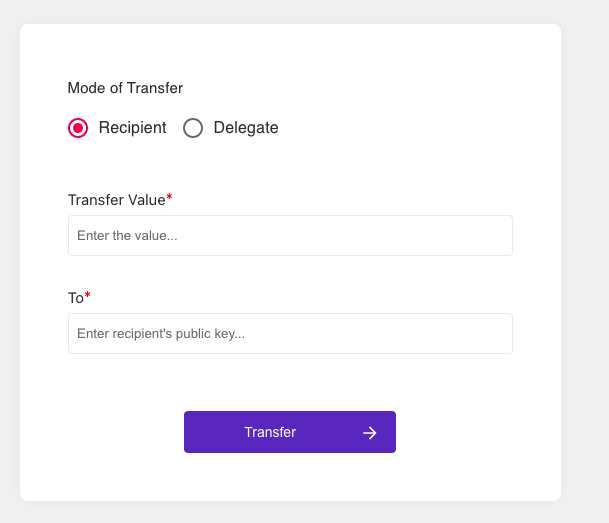
\includegraphics[width=\linewidth]{figures/images/ramu/t_transfer_recipient.png}
		  \caption{Transfer mode}
		\label{fig:ramu_ui_transfer_mode}
		\endminipage
		\hfill
		\minipage{0.45\textwidth}
		  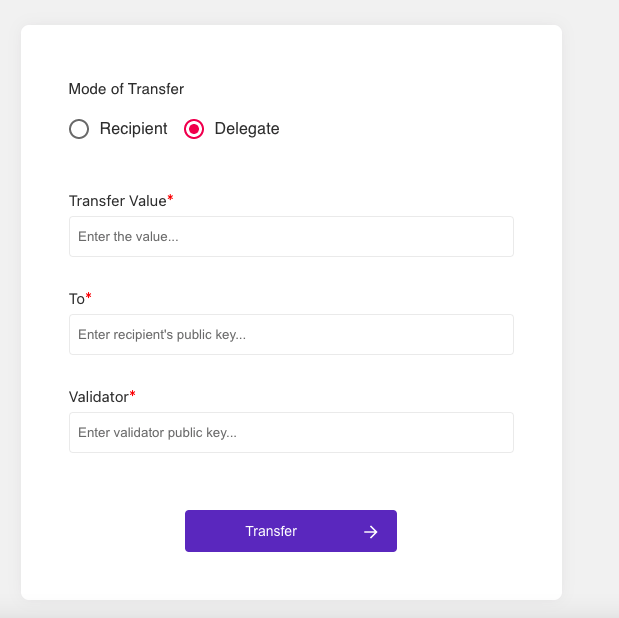
\includegraphics[width=\linewidth]{figures/images/ramu/t_transfer_delegate.png}
		  \caption{Delegate mode}
		\label{fig:ramu_ui_delegate_mode}
		\endminipage
	\end{figure}

	\item Generating a key pair: clicking on the \textit{Generate Keys} triggers the Agent to generate a key pair for the user (Figure \ref{fig:ramu_ui_balance_keys} \circled{a}).
	\begin{figure}[htbp]
		\centering
		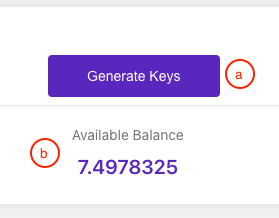
\includegraphics[width=0.3\linewidth]{figures/images/ramu/t_balance_and_keys.png}
		\caption{Balance Indicator and Generate Keys}
		\label{fig:ramu_ui_balance_keys}
	\end{figure}

	\item Balance indicator: indicates the balance with full decimal precision. Clicking the balance indicator refreshes the available balance of the agent (a cumulative sum of the values of the unspent outputs). Shown in Figure \ref{fig:ramu_ui_balance_keys} \circled{b}


	\item Manually adding a key pair: the user can add a pre-generated secret key that can be added to the Agent.
	
	\item Public keys can be chosen from the dropdown shown in Figure \ref{fig:ramu_public_keys} \circled{a}. Chosen public keys can be copied to clipboard by clicking on the copy button (Figure \ref{fig:ramu_public_keys} \circled{b}). The secret key corresponding to the selected public key is updated in the \textit{Secret Key} field (Figure \ref{fig:ramu_ui_secret_key} \circled{a}). The secret key field can be hidden or shown by clicking on the lock button (Figure \ref{fig:ramu_ui_secret_key} \circled{b}).
	
	\begin{figure}[!htb]
		\minipage{0.45\textwidth}
		  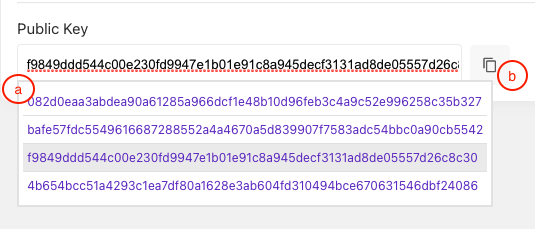
\includegraphics[width=\linewidth]{figures/images/ramu/t_public_key_selection.png}
		  \caption{Public Keys and Selection}
		\label{fig:ramu_public_keys}
		\endminipage
		\hfill
		\minipage{0.5\textwidth}
		  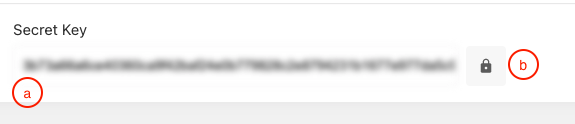
\includegraphics[width=\linewidth]{figures/images/ramu/t_secret_key.png}
		  \caption{Secret Key}
		\label{fig:ramu_ui_secret_key}
		\endminipage
	\end{figure}

	\item Additionally, confirmation dialogs and confirmation of transaction submission messages are indicated to the user.
\end{enumerate}


\begin{figure}[htbp]
    \centering
    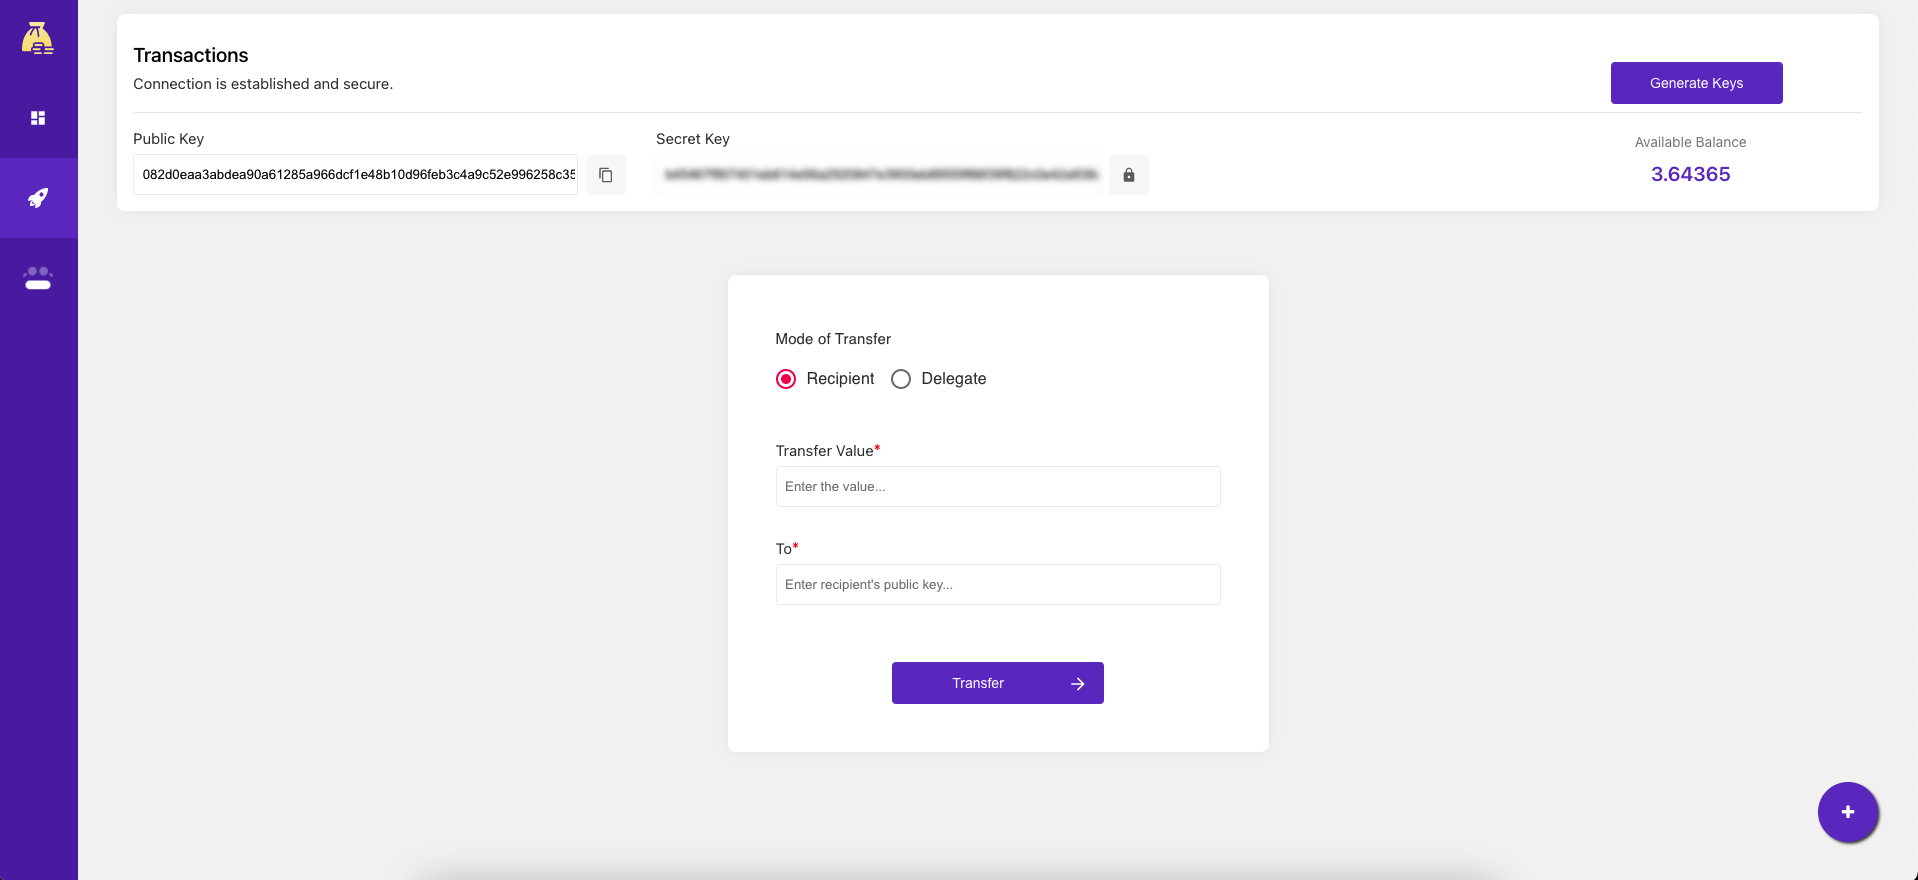
\includegraphics[width=0.8\linewidth]{figures/images/ramu/txn_page.png}
	\caption{Transactions Screen}
	\label{fig:ramu_ui_txn_screen}
\end{figure}

\subsubsection{Visualization}
The purpose of this screen is to visualize the DAG and other information graphically. A complete overview of the visualization screen is shown in Figure \ref{fig:ramu_ui_viz_screen}. Typical use cases include: 

\begin{enumerate}
	\item Visualize DAG: The portion of the screen can be zoomed in/out, click on nodes to view the information, drags and rearrange nodes. The label of the nodes shows the first 6 characters of their identifier. 
	
	In our actual implementation of the ABC protocol, only the confirmed transactions are added to the DAG and the pending transactions are maintained and tracked separately. For the purpose of visualization, the pending transactions are also included in the DAG.  
	
	The different types of nodes are shown in Figure \ref{fig:ramu_ui_viz_legend}
	\begin{figure}[htbp]
		\centering
		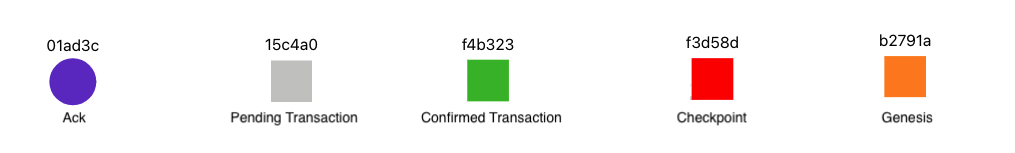
\includegraphics[width=1\linewidth]{figures/images/ramu/v_legend.png}
		\caption{Visualization Node Legend}
		\label{fig:ramu_ui_viz_legend}
	\end{figure}

	\item Hovering on the nodes indicates its predecessor(s) by highlighting the edges of the nodes that are pointing to its predecessor(s). The highlighted edges are colored in red. Figure \ref{fig:ramu_viz_complex} shows a dense DAG.
	\begin{figure}[!htb]
		\minipage{0.3\textwidth}
		  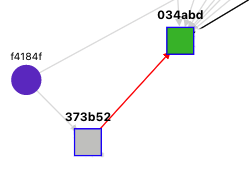
\includegraphics[width=\linewidth]{figures/images/ramu/v_txn_txn.png}
		  \caption{Transaction spending outputs of another transaction}
		\label{fig:ramu_v_txn_txn}
		\endminipage
		\hfill
		\minipage{0.3\textwidth}
		  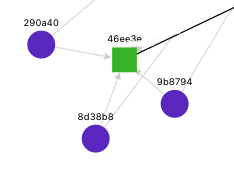
\includegraphics[width=\linewidth]{figures/images/ramu/v_ack_txn.png}
		  \caption{Acks generated for a transaction}
		\label{fig:ramu_v_ack_txn}
		\endminipage
		\hfill
		\minipage{0.3\textwidth}
		  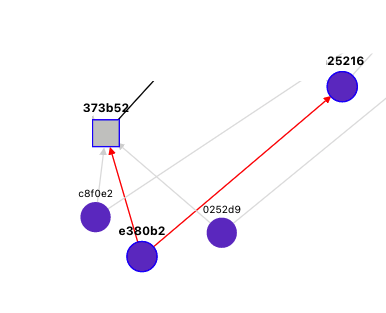
\includegraphics[width=\linewidth]{figures/images/ramu/v_ack_ack.png}
		  \caption{Ack pointing a transaction and another ack generated by the same validator}
		\label{fig:ramu_v_ack_ack}
		\endminipage
	\end{figure}

	\item Checkpoint round status is displayed at the bottom of the visualization area (Figure \ref{fig:ramu_v_ckpt_round_status}). Also, a notification is displayed when the checkpoint round status changes (Figure \ref{fig:ramu_v_ckpt_round_status_notification}).  
	\begin{figure}[!htb]
		\minipage{0.4\textwidth}
		  
\includegraphics[width=\linewidth]{figures/images/ramu/v_ckpt_status.png}
		  \caption{Checkpoint Round Status}
		\label{fig:ramu_v_ckpt_round_status}
		\endminipage
		\hfill
		\minipage{0.5\textwidth}
		  
\includegraphics[width=\linewidth]{figures/images/ramu/v_round_status_notification.png}
		  \caption{Checkpoint Round Status Notification}
		\label{fig:ramu_v_ckpt_round_status_notification}
		\endminipage
	\end{figure}

	\item Clicking on a node shows up the information corresponding to the node. Additionally, clicking on a pending transaction fetches its most recent information including its rising stake. Figures \ref{fig:ramu_v_pending_txn_info}, \ref{fig:ramu_v_confirmed_txn_info}, \ref{fig:ramu_v_ack_info}, \ref{fig:ramu_v_genesis_info}, and \ref{fig:ramu_ui_ckpt_info} show the information of the nodes for pending transaction, confirmed transaction, ack, genesis and checkpoint, respectively.
	\begin{figure}[!htb]
		\minipage{0.5\textwidth}
		  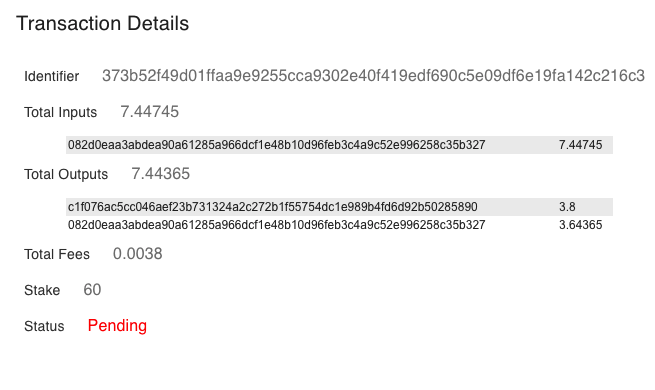
\includegraphics[width=\linewidth]{figures/images/ramu/v_pending_txn_info.png}
		  \caption{Pending Transaction}
		\label{fig:ramu_v_pending_txn_info}
		\endminipage
		\hfill
		\minipage{0.5\textwidth}
		  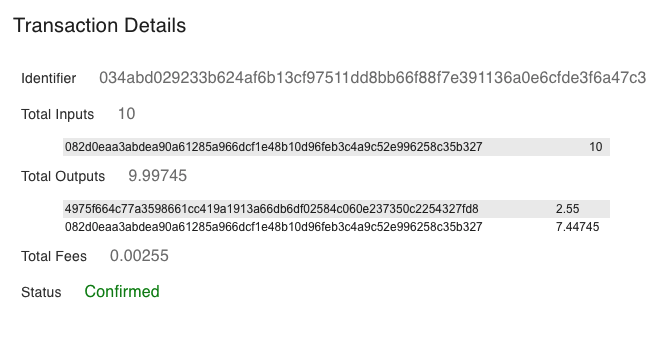
\includegraphics[width=\linewidth]{figures/images/ramu/v_confirmed_txn_info.png}
		  \caption{Confirmed Transaction}
		\label{fig:ramu_v_confirmed_txn_info}
		\endminipage
	\end{figure}
	\begin{figure}[!htb]
		\minipage{0.4\textwidth}
		  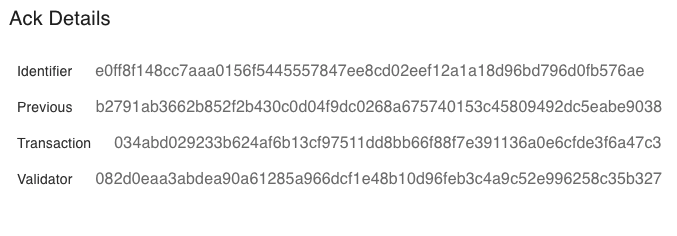
\includegraphics[width=\linewidth]{figures/images/ramu/v_ack_info.png}
		  \caption{Ack Information}
		\label{fig:ramu_v_ack_info}
		\endminipage
		\hfill
		\minipage{0.6\textwidth}
		  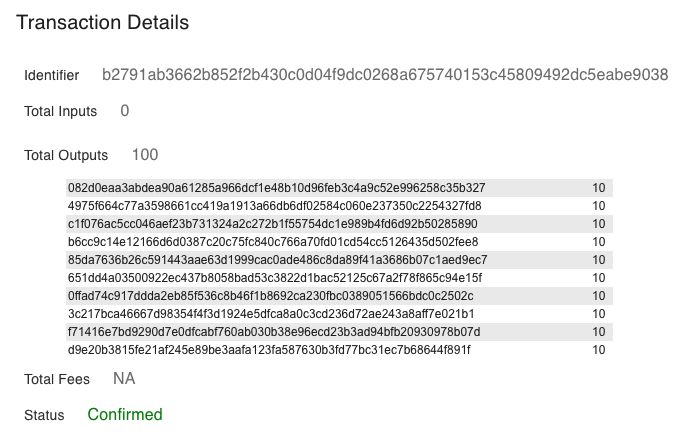
\includegraphics[width=\linewidth]{figures/images/ramu/v_genesis_txn_info.png}
		  \caption{Genesis Transaction}
		\label{fig:ramu_v_genesis_info}
		\endminipage
	\end{figure}
	\begin{figure}[htbp]
		\centering
		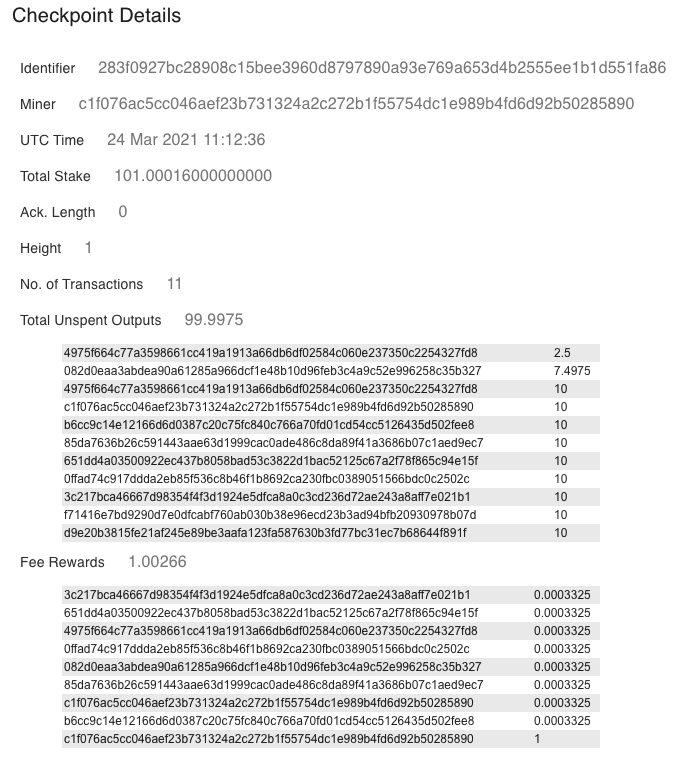
\includegraphics[width=0.8\linewidth]{figures/images/ramu/v_checkpoint_info.png}
		\caption{Checkpoint Information}
		\label{fig:ramu_ui_ckpt_info}
	\end{figure}
\end{enumerate}

\begin{figure}[htbp]
    \centering
    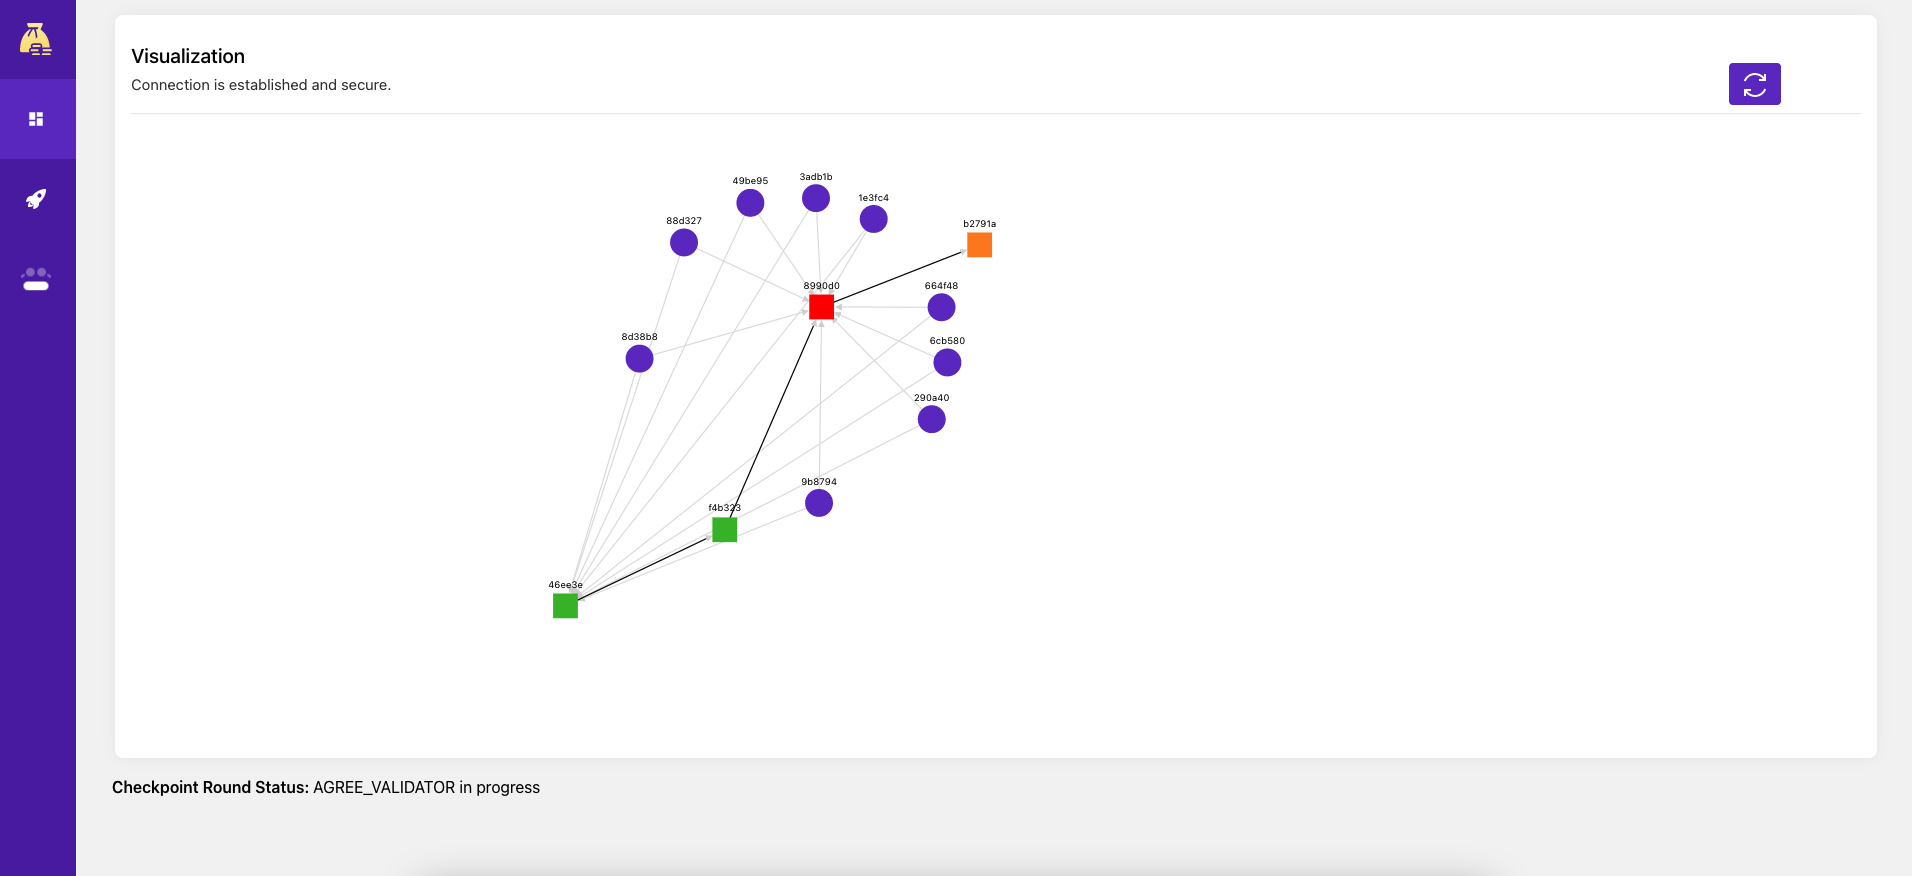
\includegraphics[width=0.8\linewidth]{figures/images/ramu/viz_page.png}
	\caption{Visualization Screen}
	\label{fig:ramu_ui_viz_screen}
\end{figure}

\begin{figure}[htbp]
    \centering
    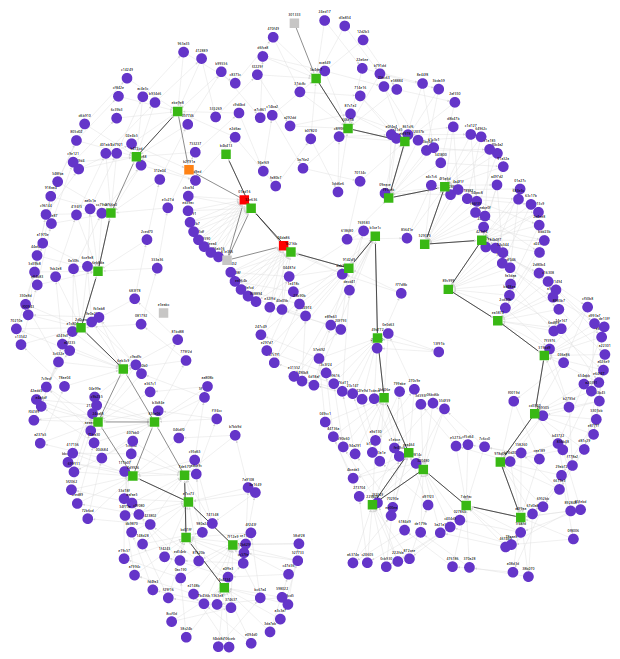
\includegraphics[width=1\linewidth]{figures/images/ramu/v_complex_viz.png}
	\caption{A glimpse of dense DAG}
	\label{fig:ramu_viz_complex}
\end{figure}

\subsubsection{Stake Distribution Chart}
The third screen showcases the stake distribution among the agents. The data for of stake distribution is collected from the checkpoint service. Figure \ref{fig:ramu_viz_stake_dist_chart} shows a overview of the stake distribution.

\begin{figure}[htbp]
    \centering
    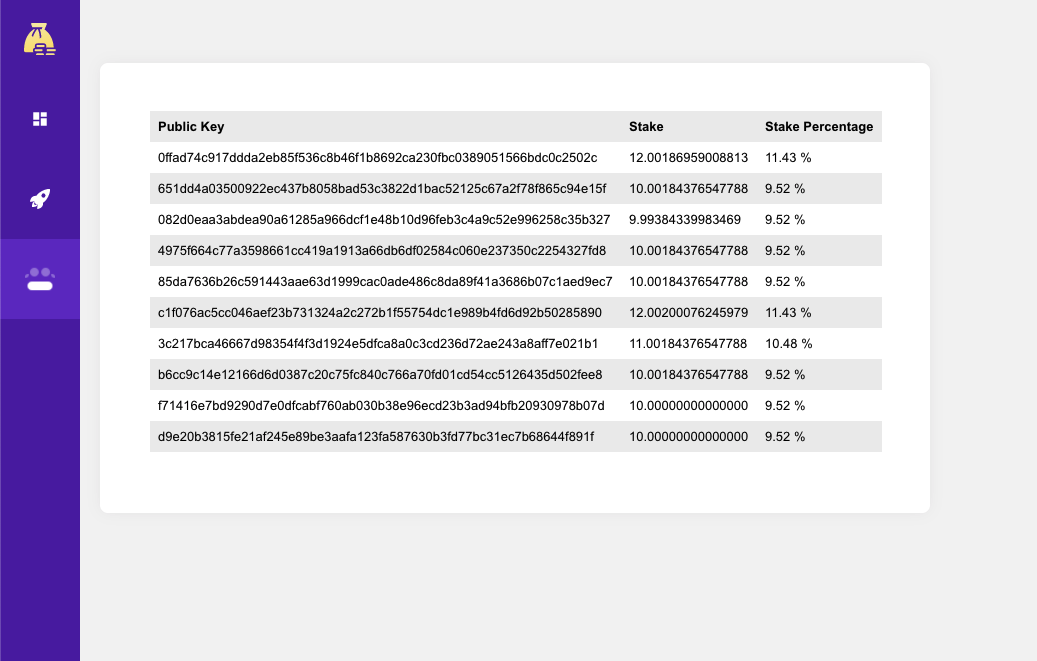
\includegraphics[width=0.8\linewidth]{figures/images/ramu/s_stake_dist_chart.png}
	\caption{Stake Distribution Chart}
	\label{fig:ramu_viz_stake_dist_chart}
\end{figure}

